\section{The Team}

%Jimmy%
\subsection{Jimmy Peleha}

\begin{figure}[t]
			\center
			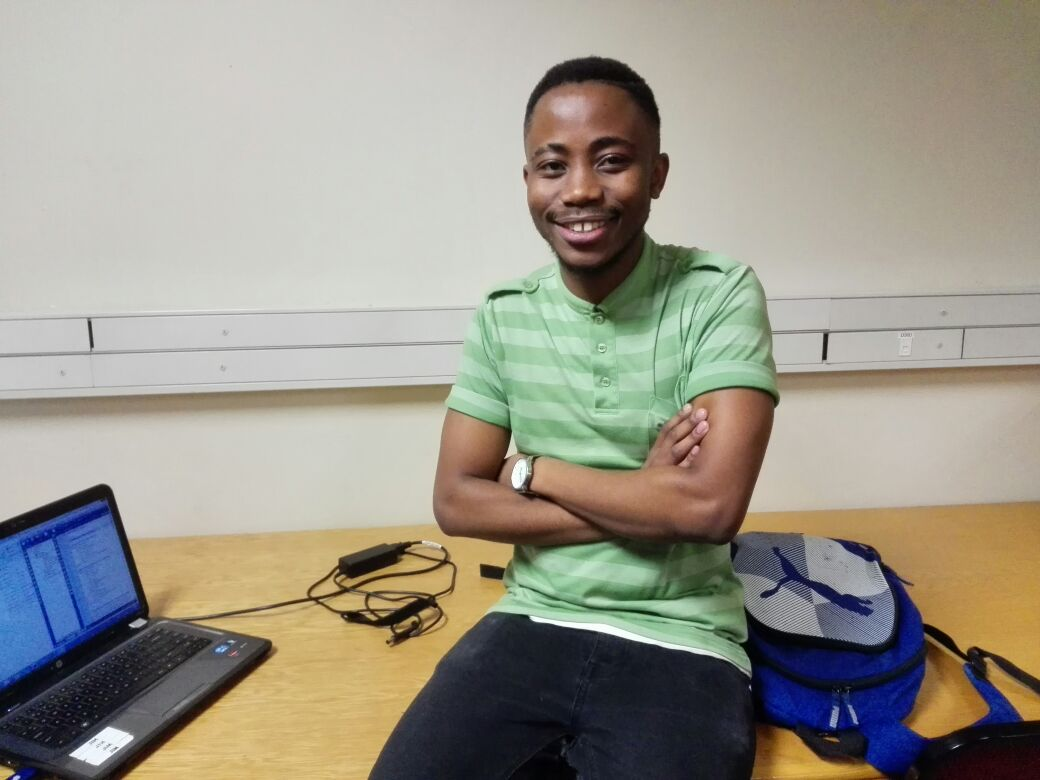
\includegraphics[width=200px]{images/Jimmy.jpg}
\end{figure}

\subsubsection{Interests:}
\begin{itemize}
	\item Chess
	\item Programming
	\item Travelling
	\item Gaming
	\item Socialising
	\item Programming Olympiads
\end{itemize}

\subsubsection{Technical Skills:}
\begin{itemize}
	\item C++
	\item Java
	\item Python
	\item C\#
	\item MySQL
	\item npm and Node.js
	\item PHP
	\item HTML, CSS
	\item XML
	\item Bootstrap
	\item Javascript
	\item Hardware Maintenance 
\end{itemize}


\subsubsection{Relevant Past Experience:}
\par{I am a two-time finalist in The Standard Bank IT Challenge. One of which my team placed third representing the University of Pretoria. This makes me confident that I can handle problems, especially in a team, whether I am under pressure or not. Synchronization and punctuality are key.}

\subsubsection{Non-Technical Strengths:}
\begin{itemize}
	\item Very approachable and charismatic
	\item Workplace experience
	\item Diligent
	\item Problem identification and solution finding
	\item Forward and straight to the point
	\item Honest
\end{itemize}

\subsubsection{Why I chose this project:}
\par{I personally have an interest in the business side of ICT. Processing large amounts of data and transforming it into information that makes a difference in the overall performance of an organization makes me feel like I've just triggered a series of well-placed dominoes. This project will have my attention effortlessly. I can learn from this project because I plan to start my own business soon.}

\newpage
%Sphe%
\subsection{Sphelele Malo}
\subsubsection{Interests:}
	\begin{itemize}
		\item Sports
		\item Security, networking and mobile development
		\item Gaming
		\item Listening and creation of music 
		\item Reading 
	\end{itemize}
\subsubsection{Technical Skills:}
	\begin{itemize}
		\item Programming
		\item Monitoring
		\item Computer and electronics 
		\item Complex problem solving
		\item Active listening
		\item Experienced with emerging technologies 
	\end{itemize}
	
\subsubsection{Relevant Past Experience:}
\par{2013 – Present: vacation work with Interfront, designing customs using agile development, and did ICT support.
}
\par{Experienced HTML, XML, SQL and even mongoDB and other emerging technologies studied during my course in the university
}
\subsubsection{Non-Technical Strengths:}
\begin{itemize}
		\item Curiosity
		\item Teamwork
		\item Communication skills
		\item Cultural fit
		\item Responsibility and initiative
	\end{itemize}
\subsubsection{Why I chose this project:}
\par{I enjoy both concurrency and web programming, combining the two, gives me an opportunity to make use of the skills I have learnt and at the same enjoy the experience. Which makes this an ideal project, not only for me but also the team. My team also shares this interest and/or view, of which is very important going forward (project development)
}

\newpage
%Armand%
\subsection{Armand Pieterse} 
\begin{figure}[h]
			\center
			\includegraphics[width=200px]{images/armand.jpg}
\end{figure}
\subsubsection{Interests:}
	\begin{itemize}
		\item Computer gaming.
		\item Programming/Software development
		\item Mixed Martial Arts
		\item Electronic Technology
	\end{itemize}
		
\subsubsection{Technical Skills:}
	\begin{itemize}
		\item C++
		\item Java
		\item	C\#
		\item	MySQL
		\item	SQLServer
		\item	MongoDB
		\item PHP
		\item HTML,CSS
		\item XML
		\item Javascript and JQuery
		\item Visual Basic 
	\end{itemize}

\subsubsection{Relevant Past Experience:}
	\par{I have experience in XML and C\# or Java which I should benefit from for this project. Although I personally don't have much experience with a Data Lake, and how it works, I am very excited to gain an understanding of it as well as learning all the technologies and strategies that goes along with it.}

\subsubsection{Non- Technical Strengths:}
	\begin{itemize}
		\item Hard Worker.
		\item Friendly and easy to work with.
		\item Perseverance
		\item Work well in a team and alone.
		\item Self-motivated.
		\item Motivating others.
	\end{itemize}

\subsubsection{Why I chose this project:}
	\par{I personally chose this project, because I have a desire to learn more about real world IT problems/challenges and how to provide a solution for it. I am at the point where I'd like to apply what I've learned so far as well as to learn more as I do so. I believe choosing RMB's project is one of the best options, because you are a respected and well-known company/bank.}

\newpage
%Sito%
\subsection{Kgomotso Sito}
\subsubsection{Interests:}
	\begin{itemize}
		\item Soccer
		\item Web programming
		\item Gaming
		\item Listening to music 
		\item Reading 
	\end{itemize}
\subsubsection{Technical Skills:}
	\begin{itemize}
		\item Programming
		\item Monitoring
		\item Operations and systems analysis
		\item Mathematics
		\item Computer and electronics 
		\item Complex problem solving
		\item Active listening
		\item Agile methodology
		\item Experienced with emerging technologies
	\end{itemize}
	
\subsubsection{Relevant Past Experience:}
\par{2013 – Present: vacation work with Interfront, designing customs using agile development, and did ICT support.
}
\par{Experienced HTML, XML, SQL and even mongoDB and other emerging technologies studied during my course in the university
}
\subsubsection{Non-Technical Strengths:}
\begin{itemize}
		\item Curiosity
		\item Teamwork
		\item Communication skills
		\item Cultural fit
		\item Responsibility and initiative
	\end{itemize}
\subsubsection{Why I chose this project:}
\par{I enjoy both concurrency and web programming, combining the two, gives me an opportunity to make use of the skills I have learnt and at the same enjoy the experience. Which makes this an ideal project, not only for me but also the team. My team also shares this interest and/or view, of which is very important going forward (project development)
}
\newpage
%Ndivhuwo%
\subsection{Ndivhuwo Nthambeleni}
\begin{figure}[h]
			\center
			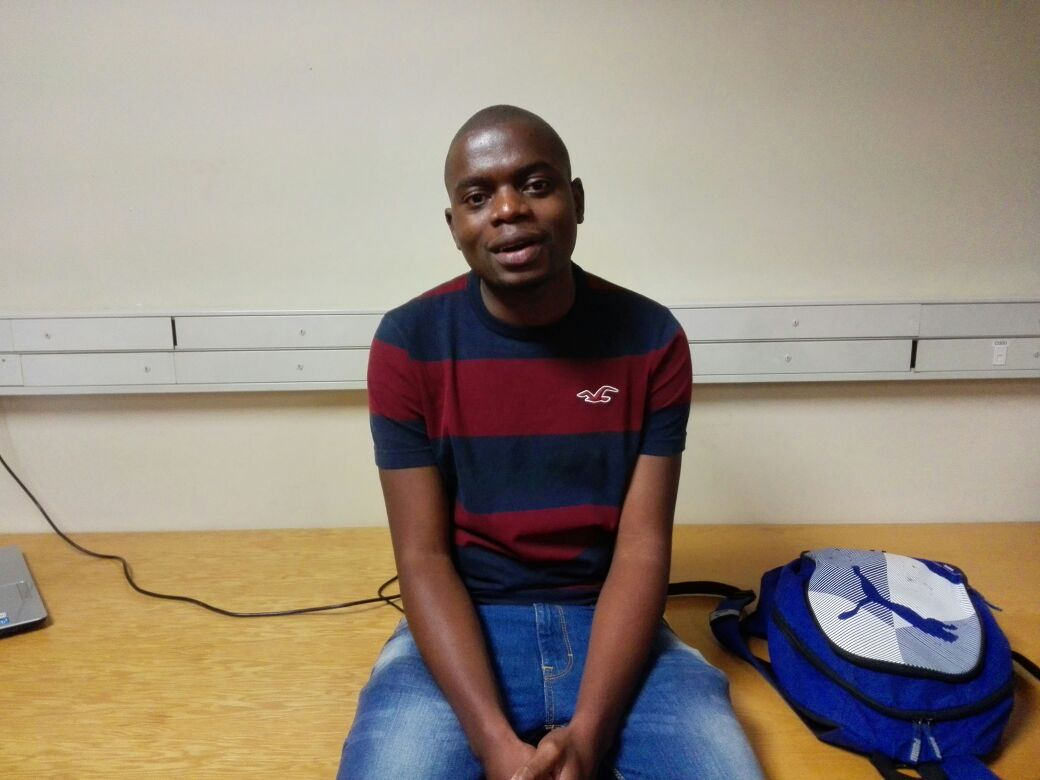
\includegraphics[width=200px]{images/Ndivhuwo.jpg}
\end{figure}
\subsubsection{Interests:}
\begin{itemize}
		\item Playing Bass guitar.
		\item Mobile development
		\item Soccer
		\item Gaming
	\end{itemize}

\subsubsection{Technical Skills:}
\begin{itemize}
		\item Programming (C++, Java, C\#, PHP (Object Oriented), HTML5, JQUERY, Python and MySQL) 1 to 4 years.
		\item Programming within the MVC, layered and Micro Kernel architectural patterns.
		\item Android Mobile Application Development 2 year
		\item Coding within the python Django and node.js frameworks.
		\item Tutoring up to 1 year
		\item Working with Linux 
		\item MS Server
		\item Advanced computer skills.
	\end{itemize}

\subsubsection{Relevant Past Experience:}
\begin{itemize}
		\item I have worked with the programming languages mentioned above for 3 years and I am quiet willing to learn new technologies that I do not have experience in.
\end{itemize}
\subsubsection{Non-Technical Strengths:}
\begin{itemize}
		\item Great Communication skills (verbal and written)
		\item Can adapt to new working environments easily.
		\item Good at identifying patterns that lead to problem solving.
\end{itemize}
\subsubsection{Why I chose this project:}
\par{I chose this project because I am looking forward to learning new technologies and enhancing my programming skills as well as applying the knowledge I have to solve problem space for this project.}
\newpage